\documentclass[conference]{IEEEtran}
\IEEEoverridecommandlockouts
\usepackage[T1]{fontenc}
\usepackage[utf8]{inputenc}
\usepackage{cite}
\usepackage{url}
\usepackage{hyperref}
\usepackage{booktabs}
\usepackage{array}
\usepackage{tabularx}
\usepackage{makecell}
\usepackage{enumitem}
\usepackage{tikz}
\usetikzlibrary{arrows.meta,positioning,shapes.geometric,fit,calc}
\usepackage{amsmath}
\usepackage{graphicx}
\usepackage{xcolor}
\usepackage{balance}
\hypersetup{hidelinks}
\setlist[itemize]{leftmargin=*, itemsep=1pt, topsep=2pt}
\setlist[enumerate]{leftmargin=*, itemsep=1pt, topsep=2pt}
\newcolumntype{Y}{>{\raggedright\arraybackslash}X}
\newcolumntype{P}[1]{>{\raggedright\arraybackslash}p{#1}}
\newcommand{\repo}{\path{raichiiiiiii/Blockchain-Based-E-Procurement-System}}
\newcommand{\mvp}{deployable staged MVP}
\tikzset{
  act/.style={rectangle, rounded corners, draw, align=center, font=\scriptsize, minimum height=7mm, text width=2.75cm},
  actwide/.style={rectangle, rounded corners, draw, align=center, font=\scriptsize, minimum height=7mm, text width=3.55cm},
  decision/.style={diamond, draw, align=center, aspect=2.3, font=\scriptsize, text width=1.55cm, inner sep=1pt},
  comp/.style={rectangle, rounded corners, draw, align=center, font=\scriptsize, minimum height=8mm, text width=3.0cm},
  store/.style={cylinder, draw, shape border rotate=90, aspect=0.28, align=center, font=\scriptsize, minimum height=10mm, text width=2.7cm},
  lane/.style={draw, rounded corners, inner sep=5pt},
  arr/.style={-Stealth, thick},
  note/.style={rectangle, draw, dashed, rounded corners, align=center, font=\scriptsize, text width=3.1cm}
}

\title{Scope Alignment and Implementation Plan for a Blockchain-Based E-Procurement System\\
\large Realigning the Existing Repository into a Business-Grounded, Deployable MVP}

\author{\IEEEauthorblockN{Prepared for Product, Engineering, QA, and Supervisor Review}
\IEEEauthorblockA{Repository: \repo\\ Date: 30 May 2026}}

\begin{document}
\maketitle

\begin{abstract}
This report realigns the existing Blockchain-Based E-Procurement System without restarting it. The product should be framed as a compliance-first procurement evidence and procurement-linked PLS financing seedbed. Procurement means requesting, ordering, delivering, invoicing, verifying, and settling goods or services. Procure-to-pay means the flow from purchase order to delivery evidence, invoice, approval, settlement status, and audit record. Blockchain proof means a tamper-evidence mechanism for selected hashes and lifecycle events, not a replacement for the operational record. The implementation plan preserves the current React, Fastify, PostgreSQL, and Hyperledger Fabric proof-anchoring foundation, then stages delivery around actor-complete procurement workflows, KYC/AML eligibility, escrow release readiness, PLS/Shariah review, audit proof, signed export bundles, and operator readiness.
\end{abstract}

\begin{IEEEkeywords}
e-procurement, procure-to-pay, Hyperledger Fabric, proof anchoring, PostgreSQL, PLS, mudarabah, Shariah governance, React, Fastify, MVP, UML
\end{IEEEkeywords}

\section{Executive Summary}
The current work should not be restarted. The repository already contains a useful foundation: a React/Vite frontend, a Fastify backend, session-based authentication, role navigation, PostgreSQL-capable persistence, procurement lifecycle events, delivery evidence, blockchain anchor APIs, escrow routes, export bundle routes, PLS routes, document routes, payment adapters, ERP/accounting routes, security routes, and deployment runbooks. The main problem is not the absence of code; it is product alignment.

The clearest product direction is:
\begin{quote}\itshape
A compliance-first procurement evidence platform for regulated buyer-supplier transactions, with optional procurement-linked PLS financing support, where sensitive business records stay in PostgreSQL/off-chain storage and selected lifecycle-event hashes are anchored to Hyperledger Fabric for audit proof.
\end{quote}

The recommended canonical MVP case is: Amanah Retail procures from Barakah Supplies; compliance verifies KYC/AML eligibility; the supplier accepts the order; escrow is created and later prepared for settlement instruction after delivery evidence; Shariah reviews the PLS terms where financing is used; Mabrur Finance reviews the PLS evidence; the auditor verifies blockchain proof; the regulator exports a signed evidence bundle. This case preserves existing work and gives every mandatory actor a concrete business job.

The primary implementation decision is to complete a staged web MVP before mobile. The frontend is already React-based, so the recommendation is not a rewrite. The correct path is an incremental React refactor around role-specific workspaces, shared state models, typed API clients, design tokens, and Figma-aligned screen flows. React Native can follow later by sharing domain types, API clients, validation rules, and design tokens, not by prematurely splitting engineering capacity.

\section{Source Reliability and Reading Order}
Implementation decisions should be guided by current repository artifacts first. Research PDFs explain the business and finance background, but they must not override current architecture contracts or code. Table~\ref{tab:source-reliability} gives the reading order.

\begin{table*}[t]
\caption{Source reliability classification and implementation use}
\label{tab:source-reliability}
\scriptsize
\begin{tabularx}{\textwidth}{P{2.5cm} P{4.1cm} Y Y}
\toprule
Class & Sources & How to use & Caution \\
\midrule
Current source of truth & \path{src/}, \path{package.json}, \path{docs/analysis/CURRENT_PRODUCT_TECHNICAL_REQUIREMENTS_META_ANALYSIS.md}, \path{docs/architecture/}, \path{docs/contracts/}, \path{backlog/backlog.csv}, \path{backlog/production-extension-roadmap.csv}, \path{backlog/plan.mermaid} & Use for scope, implemented boundaries, APIs, state models, role rules, persistence, demo readiness, acceptance criteria, and Codex tasks. & Resolve contradictions in favor of current contracts/code plus explicit boundary documents. \\
Supporting research & \path{procurement_thesis_final.pdf}, \path{mudarabah_performance_report_malaysia.pdf}, \path{blockchain_hyperledger_fabric_thesis.pdf}, \path{mudarabah_procurement_thesis.pdf} & Use to define procurement inefficiencies, P2P stages, blockchain fit, and why mudarabah needs evidence, accounting, and monitoring. & These are explanatory; they do not define repository APIs. \\
Historical or premature material & \path{IEEE FYP1 1625 D.pdf} & Use for origin context: hybrid architecture, financier read-only audit view, and transparency-layer idea. & Treat commit-reveal/tender-heavy scope as historical unless current backlog confirms it. Do not use it as current implementation truth. \\
Implementation evidence & \path{docs/evidence/}, smoke tests, QA files, runbooks & Use to validate completed PBIs and UAT readiness. & Evidence files prove tests/acceptance at a time; they are not contracts unless linked by architecture/contracts docs. \\
Draft or superseded material & Formal reports and old proposals under \path{docs/report/} and \path{docs/proposals/} when not aligned to current contracts & Use for narrative, supervisor reporting, and traceability. & Label superseded claims. Do not claim production payment, formal Shariah certification, or full Fabric consortium unless implemented. \\
\bottomrule
\end{tabularx}
\end{table*}

The highest-value reading order for a coding agent is: (1) README and runbooks, (2) current technical meta-analysis, (3) architecture boundary documents, (4) contracts, (5) source code modules, (6) backlog CSVs, (7) QA evidence, then (8) supporting PDFs.

\section{Real Business Problem}
Traditional procurement creates problems when orders, delivery proof, invoices, approvals, payment status, supplier records, and audit evidence are spread across email, spreadsheets, disconnected systems, and manual approvals. The affected parties are buyers who need controlled purchasing; suppliers who need predictable order and payment status; compliance teams who must know whether organizations are eligible; financiers who need reliable evidence before supporting procurement-linked financing; Shariah reviewers who need traceable PLS terms; auditors and regulators who need evidence without broad disclosure of private records.

\textbf{Concise problem statement.} Regulated procurement participants need one reliable case file for onboarding, purchase order acceptance, delivery proof, escrow release readiness, financing review, Shariah governance, audit proof, and evidence export. The system should reduce fragmented evidence and trust friction by recording procurement lifecycle events off-chain, protecting access by role, and anchoring selected hashes to a permissioned blockchain for verification. It should not pretend that blockchain proves the real-world truth of delivery, executes bank payments, or automatically makes PLS Shariah-compliant.

MVP-critical problems are identity/session control, role-based access, KYC/AML eligibility, buyer-supplier order workflow, escrow creation and release-readiness state, delivery evidence, transaction history, proof verification, and export evidence. Production-extension problems are full DID federation, production Fabric consortium, ISO 20022 bank execution, tokenized receivables, IoT/EPCIS device networks, legal hold automation, formal Shariah certification, and multi-jurisdiction governance.

\section{Product Scope Statement}
\textbf{In scope for staged MVP:}
\begin{itemize}
  \item public product entry, login, session handling, and role-based dashboards;
  \item organization registration, membership status, role assignment, and access history;
  \item KYC/AML onboarding and eligibility gates;
  \item buyer order workspace, supplier received orders, order acceptance, delivery evidence, invoice/receivable references, escrow creation, and settlement-instruction readiness;
  \item PLS/mudarabah support as a governed financing record, not live capital movement;
  \item Shariah review checklist, decision, conditions, and certificate metadata where implemented;
  \item transaction history, audit events, blockchain proof viewer, proof verification, and export bundle workflow;
  \item local/containerized deployment, smoke test, seeded demo accounts, UAT scripts, and supervisor demo evidence.
\end{itemize}

\textbf{Out of scope for the MVP:}
\begin{itemize}
  \item production payment execution or bank settlement;
  \item production Fabric consortium operations unless explicitly staged as extension;
  \item raw sensitive business data, KYC data, payment credentials, or unrestricted contract text on-chain;
  \item automated Shariah compliance, legal advice, or binding regulatory certification;
  \item token marketplace operations or receivables trading;
  \item mobile implementation before the web MVP is stable.
\end{itemize}

\section{Actors and Stakeholders}
Actors operate the system. Stakeholders are affected by the system or integrate with it but may not use the core UI. Table~\ref{tab:actors} defines the minimum actor model.

\begin{table*}[t]
\caption{Actors, responsibilities, permissions, and data boundaries}
\label{tab:actors}
\scriptsize
\begin{tabularx}{\textwidth}{P{2.3cm} P{3.5cm} P{3.7cm} Y Y}
\toprule
Actor & Real-world responsibility & System responsibility & Can see & Must not see / must not do \\
\midrule
Visitor & Understand product and request access & View landing page, product explanation, sign-in path & Public product copy, demo entry explanation & Private cases, proof metadata, role dashboards \\
SME / Organization applicant & Register an organization and submit onboarding evidence & Create registration/KYC request, upload metadata, track status & Own organization status, requested evidence status & Other organizations' KYC files or commercial records \\
Buyer & Procure goods/services and verify delivery & Create order, send to supplier, review delivery evidence, create escrow/release request & Own orders, linked supplier safe identifiers, delivery proof metadata, escrow/proof status & Supplier private finance terms, unrelated KYC, other buyers' orders \\
Supplier & Fulfill accepted orders & Acknowledge/order response, submit delivery evidence, view escrow status & Received orders, delivery evidence, own invoice/receivable references, escrow status & Buyer internal approvals, financier-only terms, other suppliers' data \\
Administrator & Govern organizations, users, and roles & Manage members, status, role assignments, access requests & Organization/member status, role assignments, access history & Raw payment credentials; cannot bypass audit capture \\
Compliance reviewer & Determine KYC/AML eligibility & Review onboarding case, record approve/flag/block, publish eligibility decision & KYC/AML evidence metadata and decision rationale as authorized & Unauthorized commercial terms; cannot alter procurement facts \\
Shariah reviewer & Review PLS/mudarabah structure & Checklist, decision, conditions, certificate metadata & PLS terms needed for review, related evidence, decision history & Payment credentials, unrelated procurement data, hidden auto-approval \\
Financier / Islamic finance analyst & Review funding suitability and PLS performance evidence & Review eligible case, PLS contract, distribution evidence, proof metadata & Linked procurement, PLS terms, Shariah decision, relevant delivery/invoice status & Operational control of buyer/supplier actions, unrelated cases \\
Auditor & Verify audit trail and proof integrity & Query events, verify hashes, inspect completeness and access history & Lifecycle events, proof metadata, export bundle integrity & Raw KYC/payment data unless authorized; no business-state edits \\
Regulator & Request/review evidence package & Request/export signed bundle, verify manifest/proofs & Approved bundle contents and proof metadata & Broad live access to private operational data outside mandate \\
Security operator & Monitor denied access and proof failures & View alerts, investigate denied actions, escalate incidents & Security events, safe actor labels, proof failure metadata & Raw private business content unless incident policy permits \\
Operations lead / platform operator & Keep deployment running & Health/readiness, runbooks, backups, smoke tests, incident handling & Operational status, logs per policy, readiness & Business decisions; must not fabricate proof \\
Arbitrator & Resolve disputed escrow cases & Record arbitration outcome and reason when dispute module enabled & Dispute case evidence and escrow status & Unrelated KYC/finance records \\
Developer & Build and test safely & Follow contracts, run tests, update docs/evidence & Source code, docs, local demo data & Production secrets, unauthorized personal data \\
Consortium administrator & Govern future Fabric network & Membership, endorsement policy, channel/private data rules & Network governance metadata & MVP operational state unless role-granted \\
\bottomrule
\end{tabularx}
\end{table*}

External stakeholders include regulators, banks or Islamic financial institutions, ERP/accounting systems, logistics providers, IoT/QR evidence systems, supervisors, and future consortium members. These stakeholders should be represented through explicit APIs, export bundles, or review workflows rather than informal database access.

\section{End-to-End Procurement Workflow}
Figure~\ref{fig:activity} shows the behavioral workflow. Table~\ref{tab:workflow} maps stages to triggers, outputs, audit events, proof needs, and MVP priority.

\begin{figure*}[t]
\centering
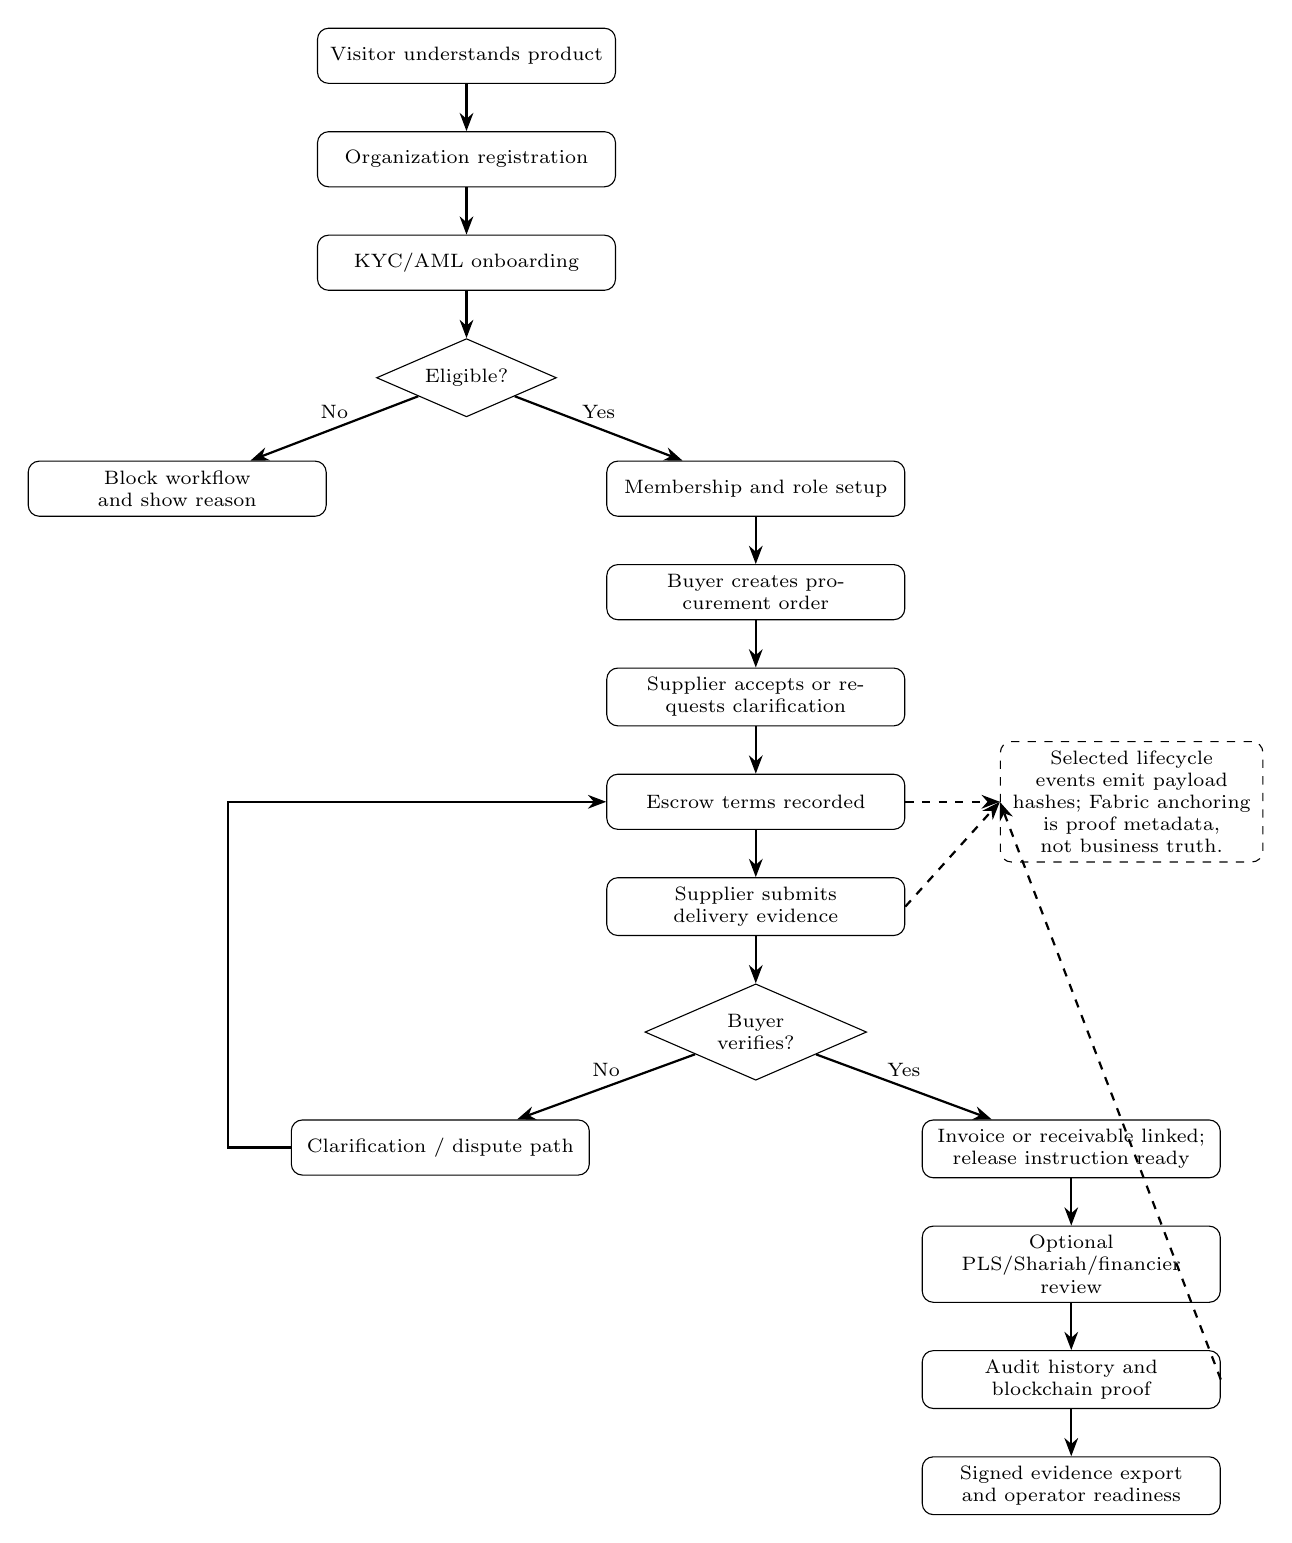
\begin{tikzpicture}[node distance=6mm and 7mm]

\node[actwide] (v) {Visitor understands product};
\node[actwide, below=of v] (reg) {Organization registration};
\node[actwide, below=of reg] (kyc) {KYC/AML onboarding};
\node[decision, below=of kyc] (elig) {Eligible?};
\node[actwide, below left=8mm and 12mm of elig] (block) {Block workflow and show reason};
\node[actwide, below right=8mm and 12mm of elig] (roles) {Membership and role setup};
\node[actwide, below=of roles] (order) {Buyer creates procurement order};
\node[actwide, below=of order] (accept) {Supplier accepts or requests clarification};
\node[actwide, below=of accept] (escrow) {Escrow terms recorded};
\node[actwide, below=of escrow] (delivery) {Supplier submits delivery evidence};
\node[decision, below=of delivery] (verify) {Buyer verifies?};
\node[actwide, below left=8mm and 14mm of verify] (clarify) {Clarification / dispute path};
\node[actwide, below right=8mm and 14mm of verify] (settle) {Invoice or receivable linked; release instruction ready};
\node[actwide, below=of settle] (pls) {Optional PLS/Shariah/financier review};
\node[actwide, below=of pls] (audit) {Audit history and blockchain proof};
\node[actwide, below=of audit] (export) {Signed evidence export and operator readiness};

\draw[arr] (v) -- (reg);
\draw[arr] (reg) -- (kyc);
\draw[arr] (kyc) -- (elig);
\draw[arr] (elig) -- node[above, font=\scriptsize]{No} (block);
\draw[arr] (elig) -- node[above, font=\scriptsize]{Yes} (roles);
\draw[arr] (roles) -- (order);
\draw[arr] (order) -- (accept);
\draw[arr] (accept) -- (escrow);
\draw[arr] (escrow) -- (delivery);
\draw[arr] (delivery) -- (verify);
\draw[arr] (verify) -- node[above, font=\scriptsize]{No} (clarify);
\draw[arr] (verify) -- node[above, font=\scriptsize]{Yes} (settle);
\draw[arr] (clarify.west) -- ++(-.8,0) |- (escrow.west);
\draw[arr] (settle) -- (pls);
\draw[arr] (pls) -- (audit);
\draw[arr] (audit) -- (export);

\node[note, right=12mm of escrow] (proofnote) {Selected lifecycle events emit payload hashes; Fabric anchoring is proof metadata, not business truth.};
\draw[arr, dashed] (escrow.east) -- (proofnote.west);
\draw[arr, dashed] (delivery.east) -- (proofnote.west);
\draw[arr, dashed] (audit.east) -- (proofnote.west);
\end{tikzpicture}
\caption{UML-style activity diagram for the realigned procurement workflow.}
\label{fig:activity}
\end{figure*}

\begin{table*}[t]
\caption{Workflow stage mapping to actor, output, audit, proof, and MVP priority}
\label{tab:workflow}
\scriptsize
\begin{tabularx}{\textwidth}{P{.5cm} P{2.4cm} P{2.2cm} P{3.2cm} P{3.2cm} P{2.5cm} P{1.4cm}}
\toprule
\# & Stage & Main actor & Trigger/input & Output & Audit/proof requirement & Priority \\
\midrule
1 & Product entry & Visitor & Landing visit & Clear product explanation and sign-in & No blockchain proof & P0 \\
2 & Registration & SME/Admin & Organization wants access & Member organization request & Access/member audit event & P0 \\
3 & Identity/KYC/AML & SME, Compliance & Onboarding evidence & Eligibility status: approved/flagged/blocked & Audit decision; documents off-chain & P0 \\
4 & Roles/membership & Administrator & Approved organization/user & Active role assignments & Access audit for changes/denials & P0 \\
5 & Buyer order & Buyer & Need to procure goods/services & Draft/sent purchase order & Lifecycle event: purchaseOrderCreated & P0 \\
6 & Supplier response & Supplier & Received PO & Accepted/rejected/clarification & purchaseOrderAccepted/Rejected & P0 \\
7 & Escrow creation & Buyer/System & Accepted order and terms hash & EscrowCreated record & Hash may be anchored & P0 \\
8 & Delivery evidence & Supplier & Goods/services delivered & Evidence metadata, documents, QR/hash refs & deliveryEvidenceSubmitted; anchor selected hash & P0 \\
9 & Buyer verification & Buyer & Evidence package & Accepted/rejected evidence & deliveryAccepted/Rejected & P0 \\
10 & Invoice/receivable link & Supplier/Buyer & Accepted delivery & Invoice/receivable reference & invoiceIssued/Approved where implemented & P1 \\
11 & Release readiness & Buyer/Admin/System & Evidence, eligibility, no dispute & settlementInstructionReady & Escrow lifecycle event; no real money movement & P0/P1 \\
12 & PLS/mudarabah & Financier/Shariah & Financing applicable & PLS contract/review/distribution scenario & Review history, proof refs if selected & P1 \\
13 & Audit/proof & Auditor & Event/case review & Proof verified/mismatch/not found & Proof query/verify; no raw private data & P0 \\
14 & Dispute/arbitration & Buyer/Supplier/Arbitrator & Evidence disagreement & Hold/refund/cancel/release decision & Escrow transition audit and proof optional & P2 \\
15 & Regulator export & Regulator/Auditor & Evidence request & Signed/hash-manifest bundle & Export manifest, proof metadata & P1 \\
16 & Operations readiness & Operator/Developer & Deployment/demo & Health, readiness, smoke/UAT evidence & Runbook logs; incident hooks & P0 \\
\bottomrule
\end{tabularx}
\end{table*}

\section{Feature and User Story Mapping}
The backlog should be reorganized around the business workflow, not treated as a flat list of blockchain ideas. Table~\ref{tab:feature-map} groups the current and planned feature set.

\begin{table*}[t]
\caption{Feature groups and MVP staging}
\label{tab:feature-map}
\scriptsize
\begin{tabularx}{\textwidth}{P{3.4cm} P{4.2cm} P{4.1cm} Y}
\toprule
Product area & Current backlog coverage & Gaps / overlaps & Stage decision \\
\midrule
Product entry, login, role dashboards & Product entry, login, dashboard, actor-ready deployment, role navigation & Ensure no implementation/PBI labels in UI; include no-role, suspended, backend unavailable states & P0 foundation \\
Membership, identity, KYC, access control & DID, KYC/AML, permissioned membership, RBAC, credential revocation, access logging & DID/VC federation and revocation are not needed for first deployable web MVP; keep session actor context authoritative & P0 for session/RBAC/KYC; DID post-MVP \\
Buyer-supplier procurement workflow & Order acceptance, product/order workspaces, shipment/receipt, delivery evidence & Need one complete order case from draft to supplier acceptance to delivery verification & P0/P1 core MVP \\
Escrow and delivery evidence & Order acceptance, escrow workflow, QR/IoT delivery proof, dispute/arbitration & Real bank movement out of scope; QR/IoT can be metadata first; dispute later unless needed for UAT & P0 creation/status; P1 release-ready; P2 arbitration \\
PLS, mudarabah, Shariah governance & PLS contract model, distribution workflow, Shariah governance, onboarding eligibility & Must frame as governed financing record and deterministic scenario, not live financial product & P1 governance; production certification later \\
Receivables and financing & Tokenized receivables, financier views, payment gateway & Tokenized receivables are high-risk extension; financing views should focus on evidence readiness & Defer tokenization; P1 financier dashboard \\
Audit, proof, transaction history & Immutable P2P audit trail, blockchain proof viewer, endorsement validation, private data controls & Need complete proof states: anchored, pending, failed, mismatch, not found; no raw private payloads & P0/P1 \\
Regulator export & Signed export bundles, audit reporting & Export path is critical to value proposition; implement hash-manifest before production key management & P1 \\
Dispute, operations, security & Dispute, access logs, non-repudiation, monitoring/incident hooks & Need denied-action review and proof failure visibility; arbitration can be staged & P1/P2 \\
ERP, accounting, payment, APIs & ERP adapter, ISO 20022 payment gateway, reconciliation, external APIs & Keep as adapter contracts and sandbox/JSON integrations; do not claim certified rails & P2/P3 production extension \\
Commercial readiness and supervisor demo & UAT, demo readiness, release validation, commercial readiness & Align demo script to one canonical case and scope-honest claims & P0/P1 \\
\bottomrule
\end{tabularx}
\end{table*}

Stories that are too technical should be reframed around actor value. For example, ``endorsement policy validation'' becomes ``Operator can see whether proof anchoring is live, simulated, failed, or unavailable.'' Duplicate proof/status stories should be merged into one proof-state model shared by escrow, audit, delivery evidence, and export bundles. Production-only stories such as consortium governance, ISO 20022 execution, tokenized receivables, and credential revocation should remain visible but deferred.

\section{Current Architecture and Technology Stack}
Figure~\ref{fig:architecture} summarizes the intended architecture.

\begin{figure*}[t]
\centering
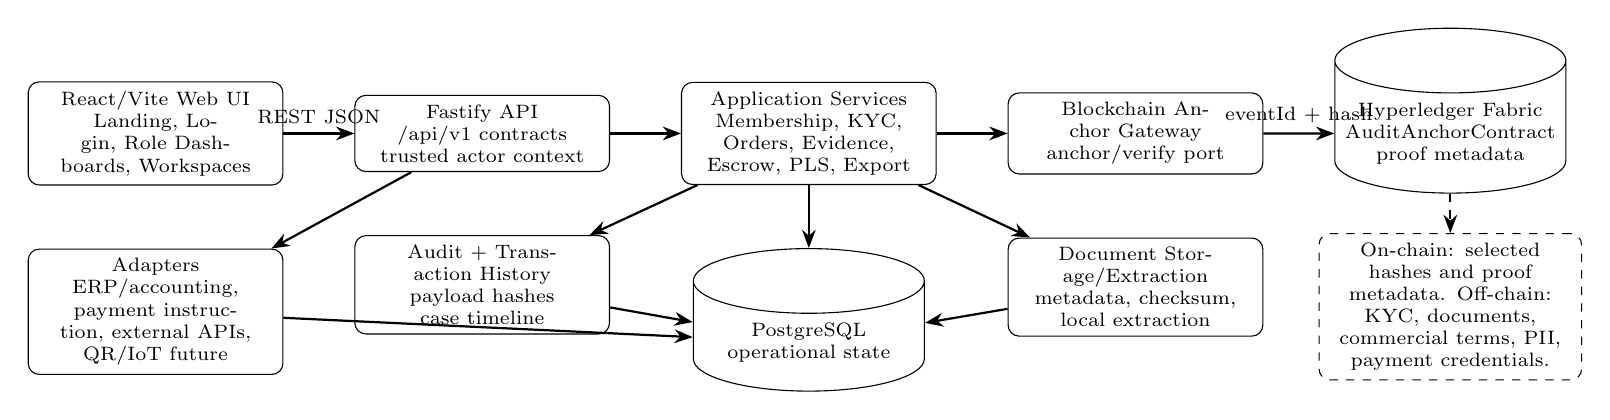
\begin{tikzpicture}[node distance=8mm and 9mm]
\node[comp] (frontend) {React/Vite Web UI\\Landing, Login, Role Dashboards, Workspaces};
\node[comp, right=of frontend] (api) {Fastify API\\/api/v1 contracts\\trusted actor context};
\node[comp, right=of api] (domain) {Application Services\\Membership, KYC, Orders, Evidence, Escrow, PLS, Export};
\node[store, below=of domain] (pg) {PostgreSQL\\operational state};
\node[comp, below=of api] (audit) {Audit + Transaction History\\payload hashes\\case timeline};
\node[comp, right=of domain] (gateway) {Blockchain Anchor Gateway\\anchor/verify port};
\node[store, right=of gateway] (fabric) {Hyperledger Fabric\\AuditAnchorContract\\proof metadata};
\node[comp, below=of gateway] (docs) {Document Storage/Extraction\\metadata, checksum, local extraction};
\node[comp, below=of frontend] (ext) {Adapters\\ERP/accounting, payment instruction, external APIs, QR/IoT future};

\draw[arr] (frontend) -- node[above, font=\scriptsize]{REST JSON} (api);
\draw[arr] (api) -- (domain);
\draw[arr] (domain) -- (pg);
\draw[arr] (domain) -- (audit);
\draw[arr] (audit) -- (pg);
\draw[arr] (domain) -- (gateway);
\draw[arr] (gateway) -- node[above, font=\scriptsize]{eventId + hash} (fabric);
\draw[arr] (domain) -- (docs);
\draw[arr] (docs) -- (pg);
\draw[arr] (api) -- (ext);
\draw[arr] (ext) -- (pg);
\node[note, below=5mm of fabric] (boundary) {On-chain: selected hashes and proof metadata. Off-chain: KYC, documents, commercial terms, PII, payment credentials.};
\draw[arr, dashed] (fabric) -- (boundary);
\end{tikzpicture}
\caption{UML-style component architecture for the staged MVP.}
\label{fig:architecture}
\end{figure*}

\textbf{Frontend.} Current stack is React, TypeScript, and Vite. The app already contains role-aware pages for administrator, buyer, supplier, compliance, Shariah, financier, auditor, regulator, and security operator, plus document and contract workspaces. Preserve this. Refactor toward case-centric screens and reusable proof/status components.

\textbf{Backend.} Current backend is Fastify with modular routes for auth, membership, access control, KYC/AML, procurement orders, delivery evidence, transaction history, blockchain anchors, escrow, export bundles, PLS, security alerts, ops status, external APIs, ERP/accounting, documents, contracts, and payments. Preserve the modular route/service/repository shape.

\textbf{Database.} PostgreSQL is the operational system of record. In-memory repositories remain useful for tests, but demos should prefer seeded PostgreSQL so state survives and operator readiness is credible.

\textbf{Authentication and RBAC.} Protected routes must use server-side session actor context. Frontend role labels must not grant privileges. Client-supplied actor identity is only scaffolding and should be eliminated from protected routes.

\textbf{Audit and transaction history.} Every procurement lifecycle action should create an event with event id, case/correlation id, lifecycle stage, event type, actor user id from trusted context, target, outcome, payload hash, and optional previous event hash. Real external timestamping and production signatures are outside MVP.

\textbf{Blockchain proof anchoring.} Hyperledger Fabric should be used as proof infrastructure for selected hashes. It should not store raw documents, KYC, payment credentials, unrestricted commercial terms, or PII. If anchoring fails, the business event still exists with proof status failed or pending.

\textbf{Escrow.} Escrow first slice is order acceptance to escrowCreated. Pilot hardening adds funded marker, release request, release approval into settlementInstructionReady, hold, dispute, and arbitration-decision states. SettlementInstructionReady is not payment execution.

\textbf{Documents.} Current document scope supports metadata intake, checksums, local storage, basic extraction, and local detached-hash signature metadata. It does not provide production document management, OCR, malware scanning, legal e-signature validation, or trust-store certification.

\textbf{PLS and Shariah.} PLS support should remain a governed financing record and deterministic scenario. Shariah review controls activation and conditions. Mudarabah should be explained as profit-and-loss sharing where one party provides capital and another manages the procurement venture; it is relevant only when procurement creates a revenue-generating transaction and documentation supports cost/revenue verification.

\textbf{Deployment.} Current deployable runbook supports a local/containerized internal pilot foundation: PostgreSQL, backend, frontend, smoke test, and demo accounts. It does not claim production Fabric, production payments, production export signing, ERP integration, ISO 20022 certification, or formal Shariah certification.

\section{Frontend Direction and React Recommendation}
The recommendation is \textbf{stage the migration incrementally inside the current React frontend}. A rewrite is not justified because the repository is already React/Vite/TypeScript and already has role-aware pages and navigation. The frontend problem is semantic workflow design, not framework absence.

\textbf{Recommended frontend path:}
\begin{enumerate}
  \item Keep React/Vite for the web MVP.
  \item Refactor page content into case-centric workspaces: order workspace, supplier response, delivery evidence, escrow detail, proof detail, KYC case, Shariah checklist, PLS contract, export bundle, and security event.
  \item Introduce shared UI primitives: status badge, proof panel, audit timeline, evidence card, role shell, empty state, forbidden state, unavailable state, and action footer.
  \item Add design tokens from the Figma prototype under \path{src/frontend/styles/tokens.css}; keep page-specific CSS thin.
  \item Create shared TypeScript domain/API types for future React Native reuse.
  \item Do not begin React Native implementation until the web MVP passes actor UAT and local deployment smoke tests.
\end{enumerate}

React supports the current web MVP and future mobile direction by allowing shared TypeScript domain models, validation rules, API clients, and design tokens. React Native should reuse workflow logic, not blindly reuse DOM components.

\section{MVP Stage Plan}
\begin{table*}[t]
\caption{Staged MVP implementation plan}
\label{tab:stage-plan}
\scriptsize
\begin{tabularx}{\textwidth}{P{2cm} P{3cm} P{4.1cm} P{4.1cm} Y}
\toprule
Stage & Goal & Included features & Excluded items & Acceptance evidence \\
\midrule
1. Scope lock and documentation alignment & Freeze product interpretation before coding & Update source reliability, actor matrix, workflow map, PBI stage labels, canonical case, README links & New production infrastructure & Updated \path{/docs}, backlog labels, ADRs, traceability table \\
2. Deployable foundation & Make app start reliably with real persisted demo state & Auth/session, role routing, PostgreSQL runtime, protected backend routes, access audit, smoke tests, deployable runbook & Fabric live network as hard dependency, real payments & \path{npm test}, typecheck, Docker smoke, demo login for all roles \\
3. Core procurement workflow & Complete buyer-supplier-escrow-delivery path & Buyer order, supplier acceptance, escrow creation, delivery evidence, buyer verification, transaction history & Tokenized receivables, full dispute automation, bank rails & UAT script for buyer and supplier; lifecycle events recorded \\
4. Governance and compliance & Make eligibility and Shariah decisions affect downstream actions & KYC/AML review, eligibility gate, Shariah checklist, PLS contract review, financier view & Formal Shariah certificate/legal opinion, production credit decisioning & Blocked/approved paths, reviewer evidence, PLS activation gating \\
5. Proof, audit, and export & Prove integrity and regulatory evidence value & Proof viewer, verify states, audit event inspection, signed/hash-manifest export bundle, regulator/auditor flow & HSM/key management, external timestamping authority & Proof verified/mismatch/not-found tests; export bundle verification \\
6. Production readiness extension & Prepare pilot hardening without overloading MVP & ERP/accounting adapter, external API gateway, observability, incident hooks, backup/rollback, docs CI, final UAT & Production consortium, ISO 20022 certification, IoT hardware rollout & Readiness checklist, incident runbook, integration contract tests \\
\bottomrule
\end{tabularx}
\end{table*}

\subsection{Codex-ready work by stage}
Each stage should produce a small pull request or commit sequence. Avoid prompts such as ``finish MVP.'' Use tasks with paths, tests, and acceptance criteria as listed in Section~\ref{sec:codex}.

\section{\texorpdfstring{\texttt{/docs} Update Recommendations}{/docs Update Recommendations}}
\begin{table*}[t]
\caption{Documentation updates}
\label{tab:docs}
\scriptsize
\begin{tabularx}{\textwidth}{P{4.2cm} P{5.4cm} Y}
\toprule
File/path & Update & Reason \\
\midrule
\path{/docs/file-index.md} & Add a maintained map of source-of-truth docs, supporting research, evidence, drafts, and runbooks & New developers need a reading order and reliability model \\
\path{/docs/DEVELOPER_ONBOARDING.md} & Add setup, architecture overview, demo users, smoke tests, coding rules, and first Codex tasks & Reduces ramp-up and prevents broad unsafe changes \\
\path{/docs/requirements/CURRENT_PRODUCT_BASELINE.md} & Define current MVP claim, actor list, excluded production claims, and canonical demo case & Locks product scope \\
\path{/docs/contracts/CONTRACT_OWNERSHIP_MATRIX.md} & Map each contract file to owner, module, tests, evidence, and backlog PBIs & Prevents orphaned contracts \\
\path{/docs/traceability/REQID_TO_PBI_TO_EVIDENCE.md} & Map requirement ids to PBIs, tests, evidence files, and demo script steps & Supports supervisor/UAT review \\
\path{/docs/contracts/CANONICAL_PAYLOAD_HASHING.md} & Resolve canonicalization drift and define one hash method used by proof, audit, export, and chaincode & Critical for proof correctness \\
\path{/docs/adr/} & Add ADRs for PostgreSQL as operational record, Fabric proof boundary, payment non-execution, and React incremental refactor & Records architecture decisions \\
\path{/docs/architecture/diagrams/} & Add rendered UML activity, sequence, component, deployment, and state diagrams & Keeps implementation visually aligned \\
\path{/docs/sprint-planning/KNOWN_LIMITATIONS_AND_POST_MVP_ROADMAP.md} & Link every deferred capability to a reason and next stage & Prevents overclaiming \\
\path{/docs/runbooks/} & Add one operator checklist for deployable MVP, backup/restore, proof failure, and demo reset & Improves repeatability \\
\path{/docs/evidence/qa/} & Add actor UAT evidence and acceptance matrix for the canonical case & Proves actor completeness \\
\bottomrule
\end{tabularx}
\end{table*}

\section{\texorpdfstring{\texttt{/backlog} Update Recommendations}{/backlog Update Recommendations}}
Backlog changes should reorganize current PBIs, not add many new features. Recommended backlog fields: \texttt{Stage}, \texttt{Actor}, \texttt{Business Process Stage}, \texttt{MVP Priority}, \texttt{Source Contract}, \texttt{Evidence Required}, \texttt{Deferred Reason}.

\textbf{Reword PBIs} that are too technical into actor/business outcomes. Example: ``Blockchain proof viewer'' becomes ``Auditor can verify that a selected procurement event hash matches the anchored Fabric proof.''

\textbf{Merge overlapping stories} around audit/proof/export states into a single proof-state model used consistently by escrow, delivery evidence, audit trail, and export bundle.

\textbf{Defer production-extension PBIs} for production Fabric consortium, ISO 20022 payment execution, tokenized receivable marketplace, credential revocation federation, IoT hardware, and multi-jurisdiction policy automation.

\textbf{Add only real-gap PBIs:}
\begin{itemize}
  \item PBI-New-01: Create source reliability and current baseline docs.
  \item PBI-New-02: Implement canonical case seed data across all mandatory actors.
  \item PBI-New-03: Add actor UAT scripts and acceptance matrix for the canonical case.
  \item PBI-New-04: Unify proof-state UI component and business-state/proof-state separation.
  \item PBI-New-05: Add traceability matrix from requirement to PBI to evidence.
\end{itemize}

\section{Codex-Ready Implementation Plan}
\label{sec:codex}
Table~\ref{tab:codex} provides concrete tasks small enough for a coding agent.

\begin{table*}[t]
\caption{Codex-ready implementation tasks}
\label{tab:codex}
\scriptsize
\begin{tabularx}{\textwidth}{P{2.6cm} P{3.2cm} P{3.5cm} P{3.5cm} Y}
\toprule
Task & Inspect & Change & Acceptance criteria & Tests/docs \\
\midrule
1. Add current baseline doc & \path{README.md}, \path{docs/analysis/}, \path{docs/architecture/}, \path{backlog/} & Create \path{docs/requirements/CURRENT_PRODUCT_BASELINE.md} & States source reliability, product claim, MVP exclusions, actors, canonical case & Link from README; no production overclaim \\
2. Add docs file index & \path{docs/} tree & Create \path{docs/file-index.md}; add README references if needed & Each major docs folder has role, status, owner, source reliability & Markdown lint/link check if available \\
3. Create traceability matrix & \path{backlog/backlog.csv}, \path{docs/contracts/}, \path{docs/evidence/} & Create \path{docs/traceability/REQID_TO_PBI_TO_EVIDENCE.md} & MVP PBIs map to contract/evidence; deferred PBIs marked with reason & Review CSV consistency \\
4. Lock canonical hashing & \path{docs/contracts/BLOCKCHAIN_ANCHOR_CONTRACT.md}, \path{docs/architecture/FABRIC_MVP_BOUNDARY.md}, source hashing utilities & Create/update \path{docs/contracts/CANONICAL_PAYLOAD_HASHING.md}; align code constants if safe & One canonicalization label used by transaction history, proof anchor, export & Unit tests for stable hash examples \\
5. Seed actor-complete case & seed scripts, auth/session repos, demo docs & Add or adjust seed for Amanah, Barakah, Mabrur, compliance, Shariah, auditor, regulator, security & All demo users log in; case visible by correct role only & \path{npm test}; deployable smoke \\
6. Remove frontend fallback drift & \path{src/frontend/lib/runtime-config.ts}, pages using fabricated data & Prefer backend seeded data where endpoints exist; keep explicit fallback disabled flag & UI shows unavailable/empty state instead of fake success & Frontend unit tests; manual role walkthrough \\
7. Complete buyer order workspace & \path{src/frontend/pages/BuyerDashboard.tsx}, procurement order routes & Add order detail/create/send flow against API & Buyer can create/send order; event recorded & API route tests; UI smoke \\
8. Complete supplier received order path & \path{SupplierDashboard.tsx}, order routes & Add list/detail/acknowledge/clarify actions & Supplier sees received orders only and can acknowledge & Authorization tests and UAT script \\
9. Unify escrow status screen & escrow routes, \path{ESCROW_WORKFLOW_CONTRACT.md}, frontend escrow nav & Display escrow status, terms hash, lifecycle event id, proof status, release readiness & Business state and proof state are distinct; no raw terms shown & Escrow tests; proof unavailable test \\
10. Delivery evidence review & delivery evidence routes, document contract, buyer/supplier pages & Supplier submits metadata; buyer accepts/clarifies & Evidence event created; raw content off-chain; buyer can review safe fields & API tests; document tests \\
11. Compliance and eligibility gate UI & KYC/AML routes, onboarding eligibility contract, ComplianceDashboard & Add case detail, decision, reason codes, downstream gate labels & Blocked org cannot create/accept gated order/escrow & Eligibility tests; UAT blocked path \\
12. Shariah/PLS activation gate & Shariah routes, PLS routes, FinancingDashboard & Show checklist, condition, approval, PLS activation blocked/ready & PLS activation requires Shariah approval/conditions & PLS route tests; UAT financier path \\
13. Proof viewer state model & blockchain anchor routes, proof UI components & Shared proof component: anchored, pending, failed, mismatch, notFound, unavailable & UI never fabricates verified proof; raw data hidden & Proof API tests; screenshot evidence \\
14. Export bundle workflow & export bundle routes, RegulatorDashboard, AuditorDashboard & Request/export/verify bundle with manifest hash and proof metadata & Regulator can view bundle status and verification result & Export tests; signed/hash manifest docs \\
15. Operator readiness & ops routes, runbooks, smoke scripts & Add readiness status page and incident hook docs & Operator can see DB/proof adapter readiness and run smoke script & Deployable smoke, runbook validation \\
16. Backlog stage labels & \path{backlog/backlog.csv}, \path{production-extension-roadmap.csv} & Add/normalize stage/priority/deferred reason columns or create companion mapping & MVP vs production extension clear to Codex and supervisor & CSV diff review; docs link \\
\bottomrule
\end{tabularx}
\end{table*}

\section{Risks, Assumptions, and Known Limitations}
\textbf{Key assumptions.}
\begin{itemize}
  \item The current repository is the active implementation base.
  \item Current docs/contracts are more reliable than early PDF drafts.
  \item PostgreSQL remains the operational record; Fabric remains proof infrastructure.
  \item The MVP is an internal pilot/supervisor-ready deployable web system, not a commercial production platform.
\end{itemize}

\textbf{Risks and controls.}
\begin{itemize}
  \item \textit{Overclaiming risk:} use ``proof anchoring'', ``settlement instruction'', and ``PLS seedbed'' instead of production blockchain/payment claims.
  \item \textit{Actor incompleteness:} finish one workflow for each mandatory actor before new infrastructure work.
  \item \textit{Privacy leakage:} keep raw KYC, documents, commercial terms, payment credentials, and PII off-chain and out of broad UI.
  \item \textit{Fabric fragility:} business events persist even when anchoring is pending or failed; readiness must disclose proof adapter state.
  \item \textit{PLS credibility:} Shariah review and deterministic records must gate financing flows; do not claim real banking or product performance.
  \item \textit{Data quality/oracle problem:} blockchain proves a hash was anchored; it does not prove a real delivery was truthful.
\end{itemize}

\section{Validation Checklist}
The realignment is valid when all checks below pass:
\begin{itemize}
  \item Current repository remains the base; no restart or parallel rewrite is introduced.
  \item Product statement is tied to procurement evidence, onboarding, order, delivery, escrow, PLS review, proof, and export.
  \item Mandatory actors have at least one defined workflow and role-specific screen.
  \item MVP and production-extension scope are separated in docs and backlog.
  \item PostgreSQL/off-chain storage is the operational source of truth; Fabric stores proof metadata only.
  \item Protected routes derive actor identity from server-side session context.
  \item Proof UI distinguishes business validity from proof availability.
  \item Sensitive data is not written raw on-chain.
  \item The web MVP is completed before React Native implementation begins.
  \item Smoke tests, UAT scripts, and evidence files demonstrate the canonical case.
\end{itemize}

\section{Follow-Up Refinement Questions}
Only these questions block final implementation prioritization:
\begin{enumerate}
  \item Should the canonical case be exactly Amanah Retail, Barakah Supplies, and Mabrur Finance, or should organization names be changed for supervisor presentation?
  \item Should direct commits to \path{main} continue, or should future Codex tasks use feature branches and pull requests?
  \item Is supervisor grading focused more on working software, formal research report, or commercial readiness narrative?
  \item Which deployment target must be demonstrated: local developer machine, Docker Compose single host, or hosted VPS?
\end{enumerate}

\section{.pdf for Download and Push .tex to Git Repository}
This report is designed as an IEEE double-column LaTeX artifact. The generated PDF should be used for supervisor and team review. The LaTeX source should be pushed under \path{docs/report/scope-alignment/} so future documentation, backlog, and implementation changes can reference a durable source file. If the repository already contains a conflicting report, create a follow-up PR rather than overwriting it without review.

\section{UML Diagram Use for Behavioral Workflow and Architectural Design}
This report includes a behavioral activity diagram in Figure~\ref{fig:activity}, an architectural component diagram in Figure~\ref{fig:architecture}, and a sequence diagram in Figure~\ref{fig:sequence}. These diagrams should also be stored as source-controlled diagram assets under \path{docs/architecture/diagrams/} in a later documentation task.

\begin{figure*}[t]
\centering
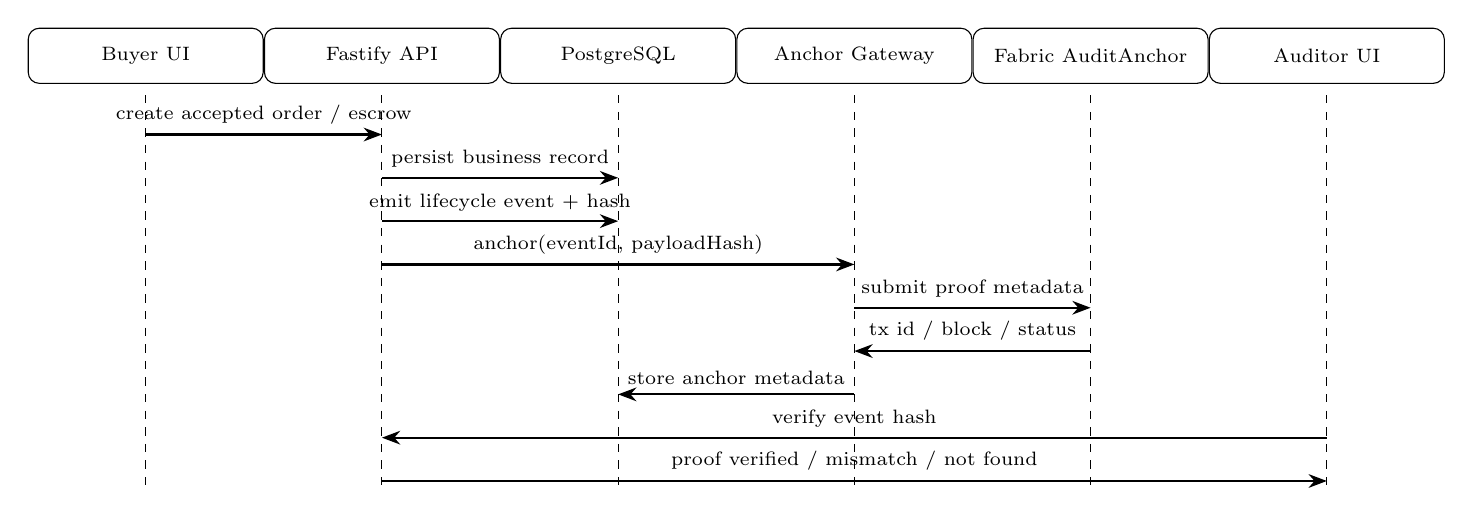
\begin{tikzpicture}[font=\scriptsize, x=1cm, y=1cm]
\node[act] (buyer) at (0,0) {Buyer UI};
\node[act] (api) at (3,0) {Fastify API};
\node[act] (db) at (6,0) {PostgreSQL};
\node[act] (gw) at (9,0) {Anchor Gateway};
\node[act] (fabric) at (12,0) {Fabric AuditAnchor};
\node[act] (auditor) at (15,0) {Auditor UI};
\foreach \x in {0,3,6,9,12,15} {\draw[dashed] (\x,-.5) -- (\x,-5.5);}
\draw[arr] (0,-1) -- node[above]{create accepted order / escrow} (3,-1);
\draw[arr] (3,-1.55) -- node[above]{persist business record} (6,-1.55);
\draw[arr] (3,-2.1) -- node[above]{emit lifecycle event + hash} (6,-2.1);
\draw[arr] (3,-2.65) -- node[above]{anchor(eventId, payloadHash)} (9,-2.65);
\draw[arr] (9,-3.2) -- node[above]{submit proof metadata} (12,-3.2);
\draw[arr] (12,-3.75) -- node[above]{tx id / block / status} (9,-3.75);
\draw[arr] (9,-4.3) -- node[above]{store anchor metadata} (6,-4.3);
\draw[arr] (15,-4.85) -- node[above]{verify event hash} (3,-4.85);
\draw[arr] (3,-5.4) -- node[above]{proof verified / mismatch / not found} (15,-5.4);
\end{tikzpicture}
\caption{UML-style sequence diagram for safe proof anchoring and verification. Business event persistence is not dependent on successful Fabric anchoring.}
\label{fig:sequence}
\end{figure*}

\section{IEEE LaTeX Format with Double Columns}
The artifact uses \texttt{IEEEtran} in conference mode. Tables and diagrams use double-column \texttt{table*} and \texttt{figure*} environments where necessary. This keeps the supervisor-facing report close to IEEE formatting while preserving practical implementation detail for developers.

\section{Conclusion}
The realignment should preserve the existing repository and narrow the product to a deployable, business-grounded procurement evidence MVP. The next engineering work should focus on source alignment, seeded actor-complete demo data, reliable PostgreSQL-backed deployment, buyer-supplier-escrow-delivery workflow completion, governance gates, proof-state correctness, export bundles, and UAT evidence. Production Fabric consortium, payment execution, tokenized receivables, IoT hardware, formal legal/Shariah certification, and React Native should remain staged extensions until the web MVP is demonstrably stable.

\balance
\begin{thebibliography}{99}
\bibitem{repo-meta} Project repository, \path{docs/analysis/CURRENT_PRODUCT_TECHNICAL_REQUIREMENTS_META_ANALYSIS.md}, \repo, 2026.
\bibitem{repo-readme} Project repository, \path{README.md}, \repo, 2026.
\bibitem{repo-fabric} Project repository, \path{docs/architecture/FABRIC_MVP_BOUNDARY.md}, \repo, 2026.
\bibitem{repo-frontend} Project repository, \path{docs/architecture/FRONTEND_PRODUCT_JOURNEY.md}, \repo, 2026.
\bibitem{repo-auth} Project repository, \path{docs/contracts/AUTH_SESSION_CONTRACT.md}, \repo, 2026.
\bibitem{repo-proof} Project repository, \path{docs/contracts/BLOCKCHAIN_ANCHOR_CONTRACT.md}, \repo, 2026.
\bibitem{repo-escrow} Project repository, \path{docs/contracts/ESCROW_WORKFLOW_CONTRACT.md}, \repo, 2026.
\bibitem{repo-history} Project repository, \path{docs/contracts/TRANSACTION_HISTORY_CONTRACT.md}, \repo, 2026.
\bibitem{repo-docs} Project repository, \path{docs/contracts/DOCUMENT_UPLOAD_EXTRACTION_CONTRACT.md}, \repo, 2026.
\bibitem{repo-runbook} Project repository, \path{docs/runbooks/deployable-mvp.md}, \repo, 2026.
\bibitem{procure-thesis} H. Irfan, \emph{Inefficiencies in Traditional Procurement and the Performance Impact of Digital Procurement Solutions}, uploaded file \path{procurement_thesis_final.pdf}, 2026.
\bibitem{mudarabah-performance} H. Irfan, \emph{Mudarabah Performance Research Report - Malaysia}, uploaded file \path{mudarabah_performance_report_malaysia.pdf}, 2026.
\bibitem{fabric-thesis} H. Irfan, \emph{Understanding Blockchain Technology and Permissioned Blockchain Applications in Hyperledger Fabric}, uploaded file \path{blockchain_hyperledger_fabric_thesis.pdf}, 2026.
\bibitem{mudarabah-procurement} H. Irfan, \emph{Understanding the Link between Mudarabah and Procurement}, uploaded file \path{mudarabah_procurement_thesis.pdf}, 2026.
\bibitem{diagnosis} H. Irfan, \emph{Research-Grade Product Diagnosis and Redesign Report for a Blockchain E-Procurement and PLS Financing Seedbed}, uploaded file \path{product_diagnosis_redesign_report.pdf}, 2026.
\bibitem{extended} H. Irfan, \emph{Extended Production Architecture and Backlog Expansion Plan}, uploaded file \path{extended_production_architecture_plan.pdf}, 2026.
\bibitem{early} H. Irfan and T. Sase, \emph{Blockchain-based Secure and Transparent E-Procurement System}, uploaded file \path{IEEE FYP1 1625 D.pdf}, historical draft, 2026.
\end{thebibliography}
\end{document}
